\section{Auswertung}
\newcommand{\tikztextc}[3]{\node at (#1, #2) {\vphantom{/}\smash{#3}};}
\newcommand{\tikztextupc}[3]{\node at (#1, #2) [rotate = 90] {\vphantom{/}\smash{#3}};}
\definecolor{myRed}{RGB}{255, 119, 94}
\definecolor{myGreen}{RGB}{140, 255, 144}
Zur Auswertung wie gut ein Analyseverfahren abschnitt, wurden zwei Klassifizierungen vorgenommen. Einmal wurden die tatsächlichen Ausreißer und Nachbarn markiert -- also die, die auf den originalen Zeitreihen erkannt wurden -- und einmal wurden die vorhergesagten Ausreißer und Nachbarn markiert -- also die, die auf den komprimierten Zeitreihen erkannt wurden. Nachdem alle Zeitreihen klassifiziert waren, konnte eine sogenannte Konfusionsmatrix erstellt werden, die Grundlage für häufig genutzte Metriken ist \cite{konfusionsmatrix}. \autoref{fig:konfusionsmatrix} zeigt wie eine solche Konfusionsmatrix aussieht. Die Klassifizierungen führen zu vier Fällen: \begin{enumerate}
    \item die Anzahl der Zeitreihen, die in den originalen und komprimierten Zeitreihen als Ausreißer / Nachbar erkannt wurden, zählen zu richtig positiv (engl. \textit{\textbf{T}rue \textbf{P}ositive}),
    \item die Anzahl der Zeitreihen, die in den originalen aber nicht in den komprimierten Zeitreihen als Ausreißer / Nachbar erkannt wurden, zählen zu falsch positiv (engl. \textit{\textbf{F}alse \textbf{P}ositive}),
    \item die Anzahl der Zeitreihen, die in den originalen und komprimierten Zeitreihen als Nicht"=Ausreißer / Nicht"=Nachbar erkannt wurden, zählen zu richtig negativ (engl. \textit{\textbf{T}rue \textbf{N}egative}),
    \item die Anzahl der Zeitreihen, die in den originalen aber nicht in den komprimierten Zeitreihen als Nicht"=Ausreißer / Nicht"=Nachbar erkannt wurden, zählen zu falsch negativ (engl. \textit{\textbf{F}alse \textbf{N}egative}).
\end{enumerate} 
Aus diesen vier Werten können nun mehrere Metriken berechnet werden, wobei für uns nur Präzision (engl. \textit{\textbf{Prec}ision}) und Genauigkeit (engl. \textit{\textbf{Acc}uracy}) von Bedeutung sind. Die Präzision berechnet sich mit der Formel \[Prec = \frac{TP}{TP + FP}\]
\begin{figure}
\centering
 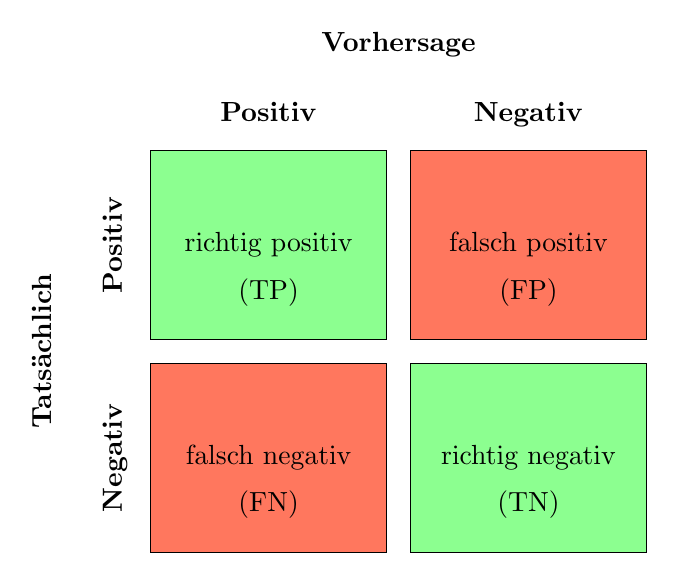
\begin{tikzpicture}[x = 3mm, y = 3mm]   % das hier verändern zum Skalieren
    % Bounding box
  \useasboundingbox (-5.2, -0.1) rectangle (21.2, 22.2);
  % links unten
  \filldraw [draw = black, fill = myRed] (0, 0) rectangle ++(10, 8);
  \tikztextc{5}{4}{falsch negativ}
  \tikztextc{5}{2}{(FN)}
  % rechts unten
  \filldraw [draw = black, fill = myGreen] (11, 0) rectangle ++(10, 8);
  \tikztextc{16}{4}{richtig negativ}
  \tikztextc{16}{2}{(TN)}
  % links oben
  \filldraw [draw = black, fill = myGreen!] (0, 9) rectangle ++(10, 8);
  \tikztextc{5}{13}{richtig positiv}
  \tikztextc{5}{11}{(TP)}
  % rechts oben
  \filldraw [draw = black, fill = myRed] (11, 9) rectangle ++(10, 8);
  \tikztextc{16}{13}{falsch positiv}
  \tikztextc{16}{11}{(FP)}
  % daneben
  \tikztextupc{-1.5}{4}{\textbf{Negativ}}
  \tikztextupc{-1.5}{13}{\textbf{Positiv}}
  \tikztextupc{-4.5}{8.5}{\textbf{Tatsächlich}}
  % drüber
  \tikztextc{5}{18.5}{\textbf{Positiv}}
  \tikztextc{16}{18.5}{\textbf{Negativ}}
  \tikztextc{10.5}{21.5}{\textbf{Vorhersage}}
 \end{tikzpicture}
 \caption{Konfusionsmatrix}
 \label{fig:konfusionsmatrix}
\end{figure}